 \chapter{Diagrama psicrom\'etrico}
 \minitoc
        \section{Par\'ametros fundamentales}
        \textbf{Aire h\'umedo.} La composici\'on del aire atmosf\'erico se lo puede simplificar como la mezcla de dos componentes: aire seco y vapor de agua.
        \begin{equation*}
            m = m_a + m_w
        \end{equation*}
        Donde
        \begin{itemize}
            \item $m_a$ la masa de aire seco
            \item $m_w$ la masa de vapor de agua
        \end{itemize}
        \textbf{Temperatura seca}($t$). Es la temperatura que registra un term\'ometro ordinario.

        \textbf{Temperatura h\'umeda}($t_h$). Es la temperatura que indica un term\'ometro cuyo bulbo est\'a cubierto por una mecha h\'umeda y expuesto a una corriente de aire. Constituye una medida indirecta del grado de humedad del aire. Si el aire no est\'a saturado, la temperatura h\'umeda es menor que la seca.

        \textbf{Humedad relativa}($\varphi$). Es la relaci\'on entre la presi\'on del vapor de agua contenido en el aire ($p_w$) y la presi\'on del vapor saturante a la misma temperatura ($p_{ws}$).

        \textbf{Humedad espec\'ifica o humedad absoluta}($W$). Es la relaci\'on entre la masa de vapor contenida en el aire ($m_w$) y la masa de aire seco ($m_a$), se expresa en $kg_v/kg_a$, es decir:
        \begin{equation*}
            W = \frac{m_w}{m_a}
        \end{equation*}
        Aplicando la ley de gases ideales y presiones parciales se puede llegar a la siguiente expresi\'on:
        \begin{equation*}
            W = 0,622\frac{\varphi\ p_{ws}(t)}{p-\varphi\ p_{ws}(t)}
        \end{equation*}
        El factor 0,622 es el resultado de dividir la constantes espec\'ificas del aire y del vapor de agua. Apartir de esta funci\'on se obtiene el \textbf{diagrama psicrom\'etrico} (\autoref{fig:diagrama-psicrometrico}).
       
        \textbf{Temperatura de roc\'io o punto de roc\'io} ($t_r$). Es la temperatura a la cual empieza la condensaci\'on del vapor de agua cuando el aire se enfr\'ia.

        \textbf{Entalp\'ia}(h). Es la cantidad de energ\'ia t\'ermica de un flujo de aire, se expresa en $kj/kg_a$. Puede determinarse a partir del diagrama psicrom\'etrico o mediante la siguiente expresi\'on:
        \begin{equation}
            h = c_{pa}\ t + W\ (h_{fg0}\ +c_{pw}\ t)
            \label{eq:entalpia}
        \end{equation}
        Donde
        \begin{itemize}
            \item $h$\ la entalp\'ia espec\'ifica en $kJ/kg_a$
            \item $c_{pa}$\ el calor espec\'ifico del aire seco en $kJ/kg_aK$
            \item $t$\ la temperatura cent\'igrada
            \item $W$\ la humedad absoluta en $kg_w/kg_a$
            \item $h_{fg0}$\ el calor latente de vaporizaci\'on del agua a 0\ \textcelsius\ en $kJ/kg_w$
            \item $c_{pw}$\ el calor espec\'ifico del vapor de agua en $kJ/(kg_w\ K)$
        \end{itemize}
        
        \textbf{Factor de calor sensible del local}(FCS). Es la relaci\'on entre la carga sensible y la carga total (sensible m\'as latente) del local.
        \begin{equation}
            FSC = \frac{\dot{Q}_S}{\dot{Q}_S\ + \dot{Q}_L}
            \label{eq:factor-calor-sensible}
        \end{equation}
        
           \begin{figure}[H]
              \centering
              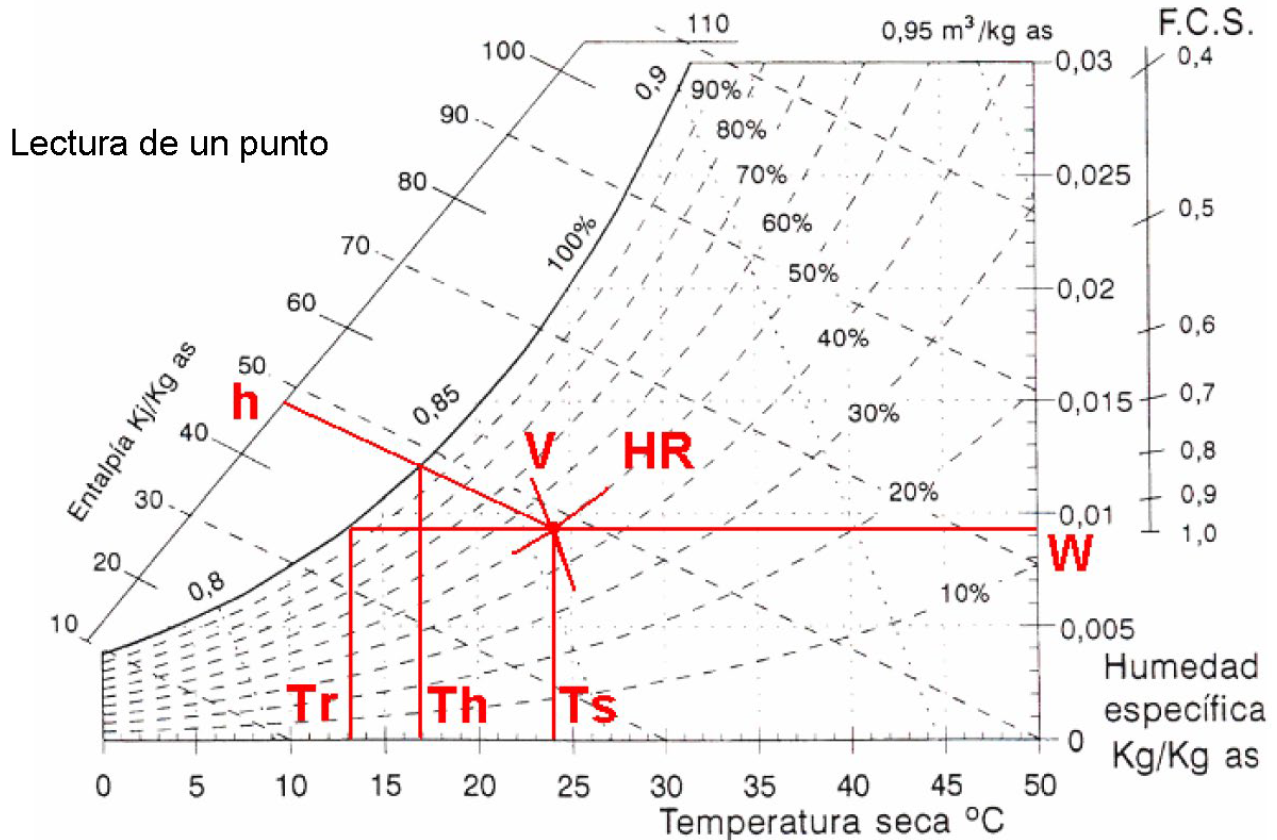
\includegraphics[width=0.5\linewidth]{psicrometrico/diagrama-psicrometrico.png}
              \caption{Diagrama psicrom\'etrico}
              \label{fig:diagrama-psicrometrico}
          \end{figure}

        \section{Operaciones b\'asicas psicrom\'etricas}

        \subsection{Mezcla de caudales}

        Esta operaci\'on se la realiza a menudo, por ejemplo, para la renovaci\'on del aire de un local. Se mezclan dos corrientes de aire de distintas temperaturas y humedades, el resultado es aire con las propiedades intermedias de las dos corrientes. Seg\'un la relaci\'on de caudales de las corrientes de entradas la mezcla tendr\'a mayor similitud con una u otra.
         \begin{figure}[H]
             \centering
             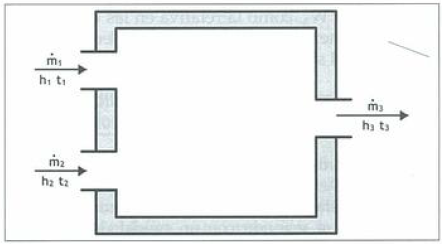
\includegraphics[width=0.5\linewidth]{psicrometrico/mezcla.png}
             \caption{Proceso de mezcla de caudales}
             \label{fig:mezcla}
         \end{figure}
        Un balance de entalp\'ias nos permite escribir:
        \begin{equation}
            \dot{m_3}\ h_3 = \dot{m_2}\ h_2\ + \dot{m_1}\ h_1
            \label{eq:balance}
        \end{equation}
        Donde
        \begin{itemize}
            \item $\dot{m_a}$\ el caudal m\'asico del flujo correspondiente
            \item $h$\ la entalp\'ia espec\'ifica del flujo
        \end{itemize}
        De \autoref{eq:balance} se puede obtener:
        \begin{equation*}
            \frac{h_3 - h_2}{h_1-h_2}=\frac{\dot{m_1}}{\dot{m_3}}
        \end{equation*}
        y de forma aproximada:
        \begin{equation*}
            \frac{t_3-t_2}{t_1-t_2}=\frac{\dot{V_1}}{\dot{V_3}}
        \end{equation*}
        de donde:
        \begin{equation}
            t_3=\frac{\dot{V_1}}{\dot{V_3}}\ (t_1-t_2)\ +\ t_2
            \label{eq:temperatura-mezcla}
        \end{equation}
         \begin{figure}[H]
             \centering
             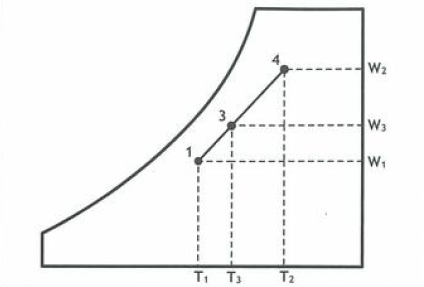
\includegraphics[width=0.5\linewidth]{psicrometrico/representacion-mezcla.png}
             \caption{Representaci\'on del proceso de mezcla}
             \label{fig:representacion-mezcla}
         \end{figure}
        Una vez obtenida la temperatura $t_3$, se sit\'ua el punto (3) en la recta 1-2 y se puede obtener tanto la humedad absoluta $W_3$, como la relativa $\varphi_3$ y la entalp\'ia $h_3$. En caso de requerir m\'as precisi\'on con el valor de la entalp\'ia se debe utilizar la \autoref{eq:entalpia}.
        
        \subsection{Calentamiento o enfriamiento sensible}

        Se trata de una operaci\'on que consiste en calentar o enfriar el aire hasta alcanzar la temperatura deseada sin modificar el contenido de humedad. Esto se puede realizar mediante resistencias el\'ectricas o un quemador de gas para el calentamiento, o haciendo pasar el aire por una bater\'ia enfriadora para enfriarlo. Este calor aportado se puede calcular de la siguiente manera:
        \begin{equation*}
            \dot{Q}=\dot{m_a}\ (h_2-h_1)
        \end{equation*}
         \begin{figure}[H]
             \centering
             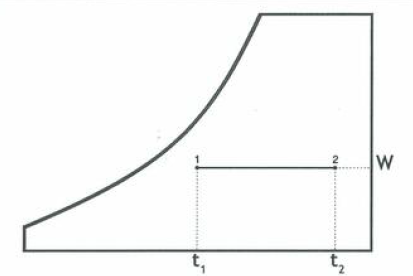
\includegraphics[width=0.4\linewidth]{psicrometrico/calentamiento-sensible.png}
             \caption{Calentamiento sensible}
             \label{fig:calentamiento-sensible}
         \end{figure}
        
        \subsection{Proceso de saturaci\'on adiab\'atica}

        Este proceso consta de hacer pasar una corriente de aire por un recinto donde hay agua, para que este vaya adquiriendo agua y salga saturado. A la entrada el aire tiene una cierta temperatura y a la salida del proceso el mismo aire tiene su temperatura de saturaci\'on o de roc\'io (\autoref{fig:representacion-saturacion-adiabatica}). Es decir, se enfr\'ia el aire añadiendole vapor de agua.
         \begin{figure}[H]
             \centering
             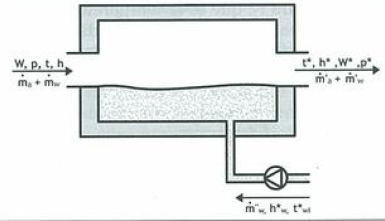
\includegraphics[width=0.4\linewidth]{psicrometrico/proceso-saturacion-adiabatica.png}
             \caption{Proceso de saturaci\'on adiab\'atica}
             \label{fig:proceso-saturacion-adiabatica}
         \end{figure}
        No hay transferencia de calor con el entorno pero si entre el agua y el aire. El agua absorbe calor para vaporizarse y el aire cede calor, disminuyendo asi su temperatura. La temperatura del aire se enfría hasta que alcanza un punto de equilibrio donde la tasa de evaporación del agua es igual a la tasa de transferencia de calor del aire al agua.
         \begin{figure}[H]
             \centering
             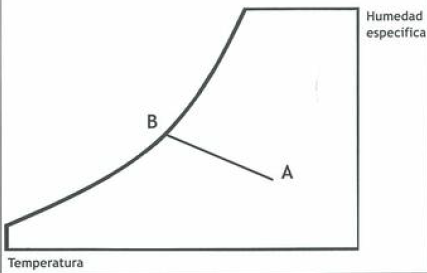
\includegraphics[width=0.4\linewidth]{psicrometrico/saturacion-adiabatica.png}
             \caption{Representaci\'on de saturaci\'on adiab\'atica}
             \label{fig:representacion-saturacion-adiabatica}
         \end{figure}

        \subsection{Humidificaci\'on}

        En esta operaci\'on se hace pasar el aire por una tela h\'umeda o una cortina de agua (spray de agua). La transformaci\'on del aire es funci\'on de la temperatura seca del aire ($T_s$), de la temperatura h\'umeda del aire ($T_h$), de la temperatura de roc\'io del aire y de la temperatura del agua ($T_{agua}$). Seg\'un los valores de estas podremos tenes:
        \begin{enumerate}
            \item $T_{agua} > T_s$, pulverizando agua caliente, o inyectando vapor de agua el aire se calienta y se humecta, por lo que su $h$ aumenta.
            \item $T_{agua} = T_s$, el aire se humecta aumentando su $h$
            \item $T_{agua} < T_s;\ T_{agua}>T_h$, el aire se enfr\'ia y se humecta, pero gana $h$
            \item $T_{agua}=T_h$, el aire se enfr\'ia y se humecta, con $h = cte$ (saturaci\'on adiab\'atica o enfriamiento evaporativo)
            \item $T_{agua}<T_h;\ T_{agua}>T_r$, el aire se enfr\'ia y se humecta perdiendo $h$
            \item $T_{agua}=T_r$, el aire se enfr\'ia sin cambio en su humedad pero pierde $h$
            \item $T_{agua}<T_r$, el aire se enfr\'ia perdiendo humedad por lo que pierde $h$
        \end{enumerate}
        En el diagrama psicrom\'etrico se pueden ver as\'i:
         \begin{figure}[H]
             \centering
             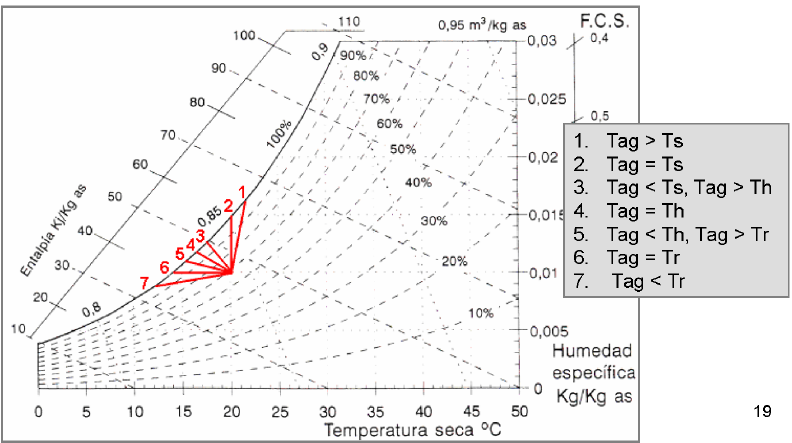
\includegraphics[width=0.6\linewidth]{psicrometrico/humidificaciones.png}
             \caption{Humidificaciones}
             \label{fig:humidificaciones}
         \end{figure}

        \subsection{Adici\'on de vapor}
        Esta transformaci\'on es \'util cuando necesitamos agregar humedad y calentar el aire, en casos de calefacci\'on por ejemplo. En el diagrama psicrom\'etrico seria de la siguiente manera:
         \begin{figure}[H]
             \centering
             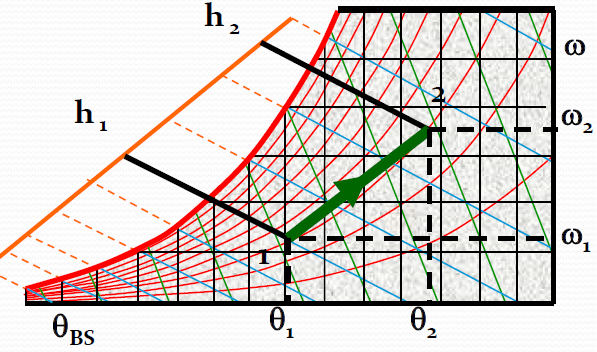
\includegraphics[width=0.5\linewidth]{psicrometrico/adicion-vapor.png}
             \caption{Adici\'on de vapor}
             \label{fig:adicion-vapor}
         \end{figure}
        
        \subsection{Deshumidificaci\'on por enfriamiento}

        El procedimiento consiste en enfriar el aire hasta una temperatura inferior a la del punto de roc\'io. Para ello, se hace pasar el aire por una bater\'ia de refrigeraci\'on, la cual est\'a constituida por un conjunto de tubos, provistos de aletas, por el interior de \'estos circula el refrigerante. 
         \begin{figure}[H]
             \centering
             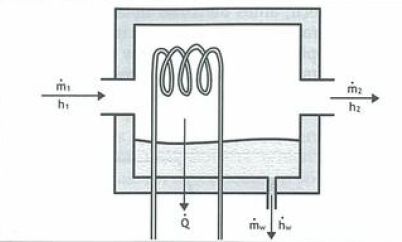
\includegraphics[width=0.4\linewidth]{psicrometrico/proceso-deshumidificacion-por-enfriamiento.png}
             \caption{Proceso de deshumidificaci\'on por enfriamiento}
             \label{fig:proceso-deshumidificacion-por-enfriamiento}
         \end{figure}
        
        \textbf{Factor de by-pass.}
        
        Observando \autoref{fig:representacion-deshumidificacion-por-enfriamiento} designemos con el n\'umero 1 las condiciones del aire de entrada, con el n\'umero 2 las condiciones del aire de salida y con el n\'umero 2' las condiciones promedio de la bater\'ia enfriadora. 
         \begin{figure}[H]
             \centering
             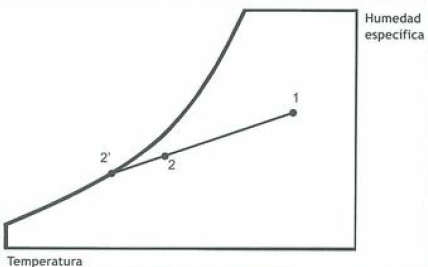
\includegraphics[width=0.4\linewidth]{psicrometrico/deshumificacion-por-enfriamiento.png}
             \caption{Representaci\'on de deshumidificaci\'on por enfriamiento}
             \label{fig:representacion-deshumidificacion-por-enfriamiento}
         \end{figure}
        El aire nunca llegar\'a a las condiciones 2' porque hay una parte de \'el que no entra en contacto con la bater\'ia. El factor de by-pass nos indica cuanta masa de aire no entra en contacto con la bater\'ia. Por lo tanto, un bajo valor de by-pass indica que nuestro dispositivo es efectivo. Este factor se representa con la letra f y se puede calcular de la siguiente manera:
        \begin{equation*}
            f = \frac{t_2-t_{2'}}{t_1-t_{2'}}
        \end{equation*}
        Donde 
        \begin{itemize}
            \item $t_2$\ temperatura a la salida
            \item $t_1$\ temperatura a la entrada
            \item $t_{2'}$\ temperatura de la superficie de la bater\'ia
        \end{itemize}
        Generalmente los fabricantes proporcionan el valor de by-pass, por lo que si despejamos de la anterior formula podemos obtener la temperatura de salida del aire:
        \begin{equation}
            t_2 = (t_1-t_{2'})\ f\ +\ t_{2'}
            \label{eq:temperatura-suministro}
        \end{equation}

        \section{Ciclo de acondicionamiento en verano}

        Una forma de extraer calor de un local es introducir fr\'io vehiculado en un fluido que en la pr\'actica suele ser uno de los casos siguientes:
        \begin{itemize}
            \item Aire fr\'io
            \item Agua fr\'ia
            \item Simult\'aneamente aire y agua
            \item Otro fluido fr\'io distinto del agua y del aire 
        \end{itemize}
        Hay que entender que, excepto en el caso del aire, tanto si se trata de agua como de cualquier otro fluido, entra y sale canalizado, sin mezclarse con el aire propio de la habitaci\'on. Cuando se emplea s\'olo aire fr\'io, \'este s\'i se mezcla con el aire de la habitaci\'on. En este caso el sistema de acondicionamiento se llama todo aire.

        El sistema de acondicionamiento \textbf{todo aire}\ el m\'etodo m\'as empleado. Consiste en mezclar aire exterior con aire procedente del local; esta mezcla se enfr\'ia en la UTA (unidad de tratamiento de aire) y se env\'ia al interior del local.
        \begin{figure}[H]
            \centering
            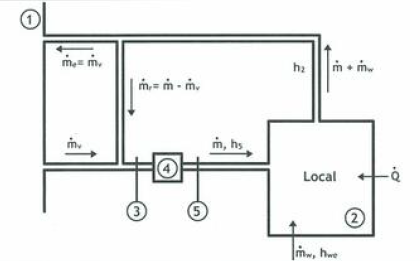
\includegraphics[width=0.6\linewidth]{acondicionamiento-ambiental/acondicionamiento-verano.png}
            \caption{Acondicionamiento por sist. todo aire}
            \label{fig:acondicionamiento-todo-aire}
        \end{figure}
        La numeraci\'on de los estados del aire en la \autoref{fig:acondicionamiento-todo-aire} es la siguiente:
        \begin{enumerate}
            \item Condiciones del aire en el exterior del local
            \item Condiciones del aire en el interior del local
            \item Condiciones del aire a la entrada de la UTA. Es el resultado de la mezclar el aire exterior con el aire procedente del local
            \item Representa una temperatura llamada punto de roc\'io de la m\'aquina, que podemos interpretar como la temperatura media de la superficie de la bater\'ia
            \item Condiciones del aire a la salida de la UTA. Este aire se llama aire de suministro
        \end{enumerate}
        Si representamos la transformaciones en el diagrama psicrom\'etrico nos quedar\'ia asi:
         \begin{figure}[H]
             \centering
             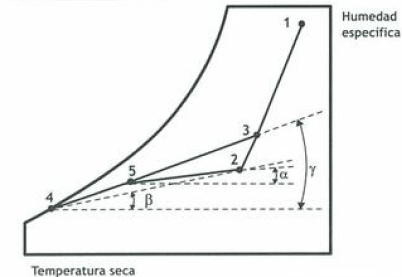
\includegraphics[width=0.4\linewidth]{psicrometrico/representacion-acondicionamiento-verano.png}
             \caption{Representaci\'on sistema todo aire}
             \label{fig:representacion-todo-aire}
         \end{figure}
        
 